\section{Application 3: Systematic Analysis}
\label{sec:app_err_analysis}


\begin{figure}[t]
\centering
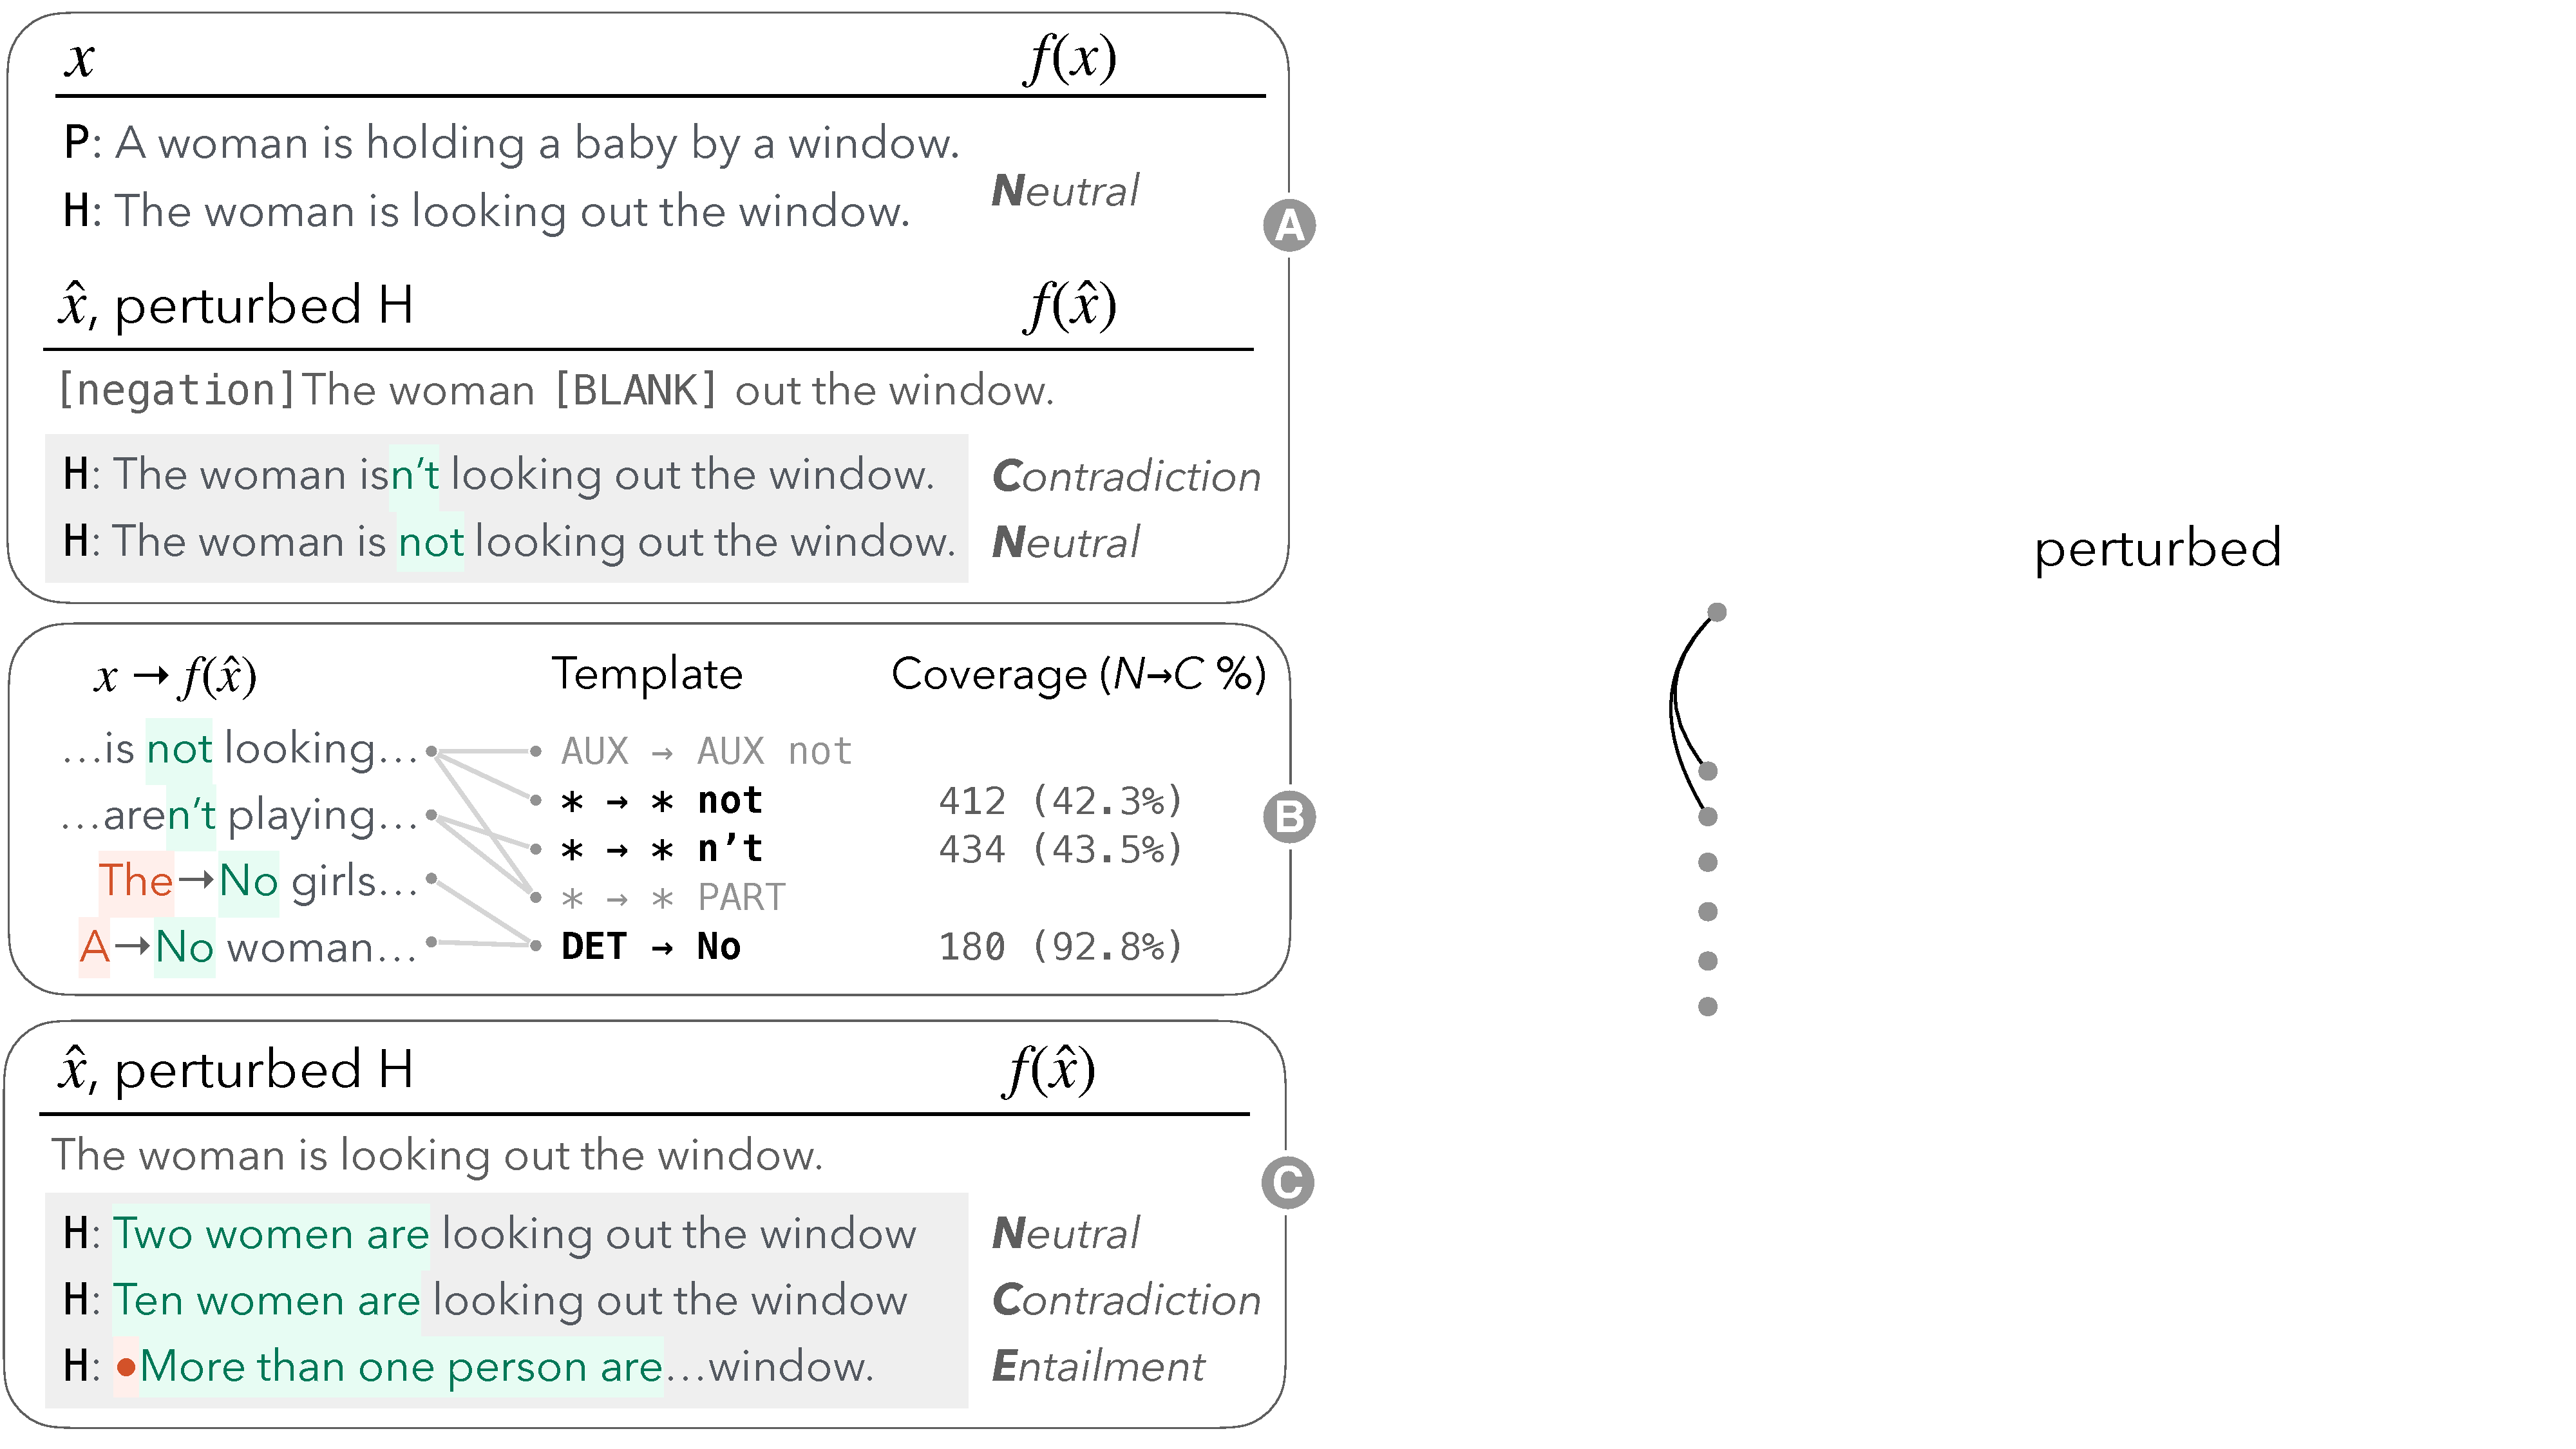
\includegraphics[trim={0 0.5cm 33cm 0cm},clip,width=1\columnwidth]{figures/err_analysis.pdf}
\vspace{-15pt}
\caption{
(A) A \qqp instance with its prediction\footnotemark showing 98.2\% confidence that the two sentences are duplicative ($=$), as well as the SHAP feature weights.
%Counterfactual explanations complement SHAP with concrete, readable examples, \eg (C) depicts a surprising flipped prediction ($\neq)$ that was missed by SHAP.
Counterfactual explanations complement SHAP with concrete, readable examples, and alert abnormalities missed by SHAP. \eg (C)
depicts a surprising flipped prediction ($\neq)$.
}
\vspace{-10pt}
\label{fig:err_analysis}
\end{figure}


Previous applications focus on a selected subset of $\xp$, but the access to the entire pool is also important.
For example, to follow up on the abnormal case in Figure~\ref{fig:explanation}C, an analyst can interactively \texttt{BLANK} ``friend'' in Q2 and observe the model's unstable behavior: it predicts \emph{Non-duplicate} when \remove{friend} is changed to \add{woman}, \add{professional}, but remains \emph{Duplicate} at \add{man}, \add{student}.
In fact, \sysname's ability to generate \emph{multiple} counterfactuals per $x$ is especially useful for systematic error analysis~\cite{wu2019errudite}.
We demonstrate such analysis through a case study on the \nli RoBERTa model in \S\ref{subsec:contrast_set}.\footnote{An additional case study is in Appendix~\ref{appendix:err_analysis_quantifier_case}.}
Here, the generation is largely driven by human analysts, and the relationship $\relation{\xp}$ can be determined by human domain expertise.
%Through a case study on the \nli RoBERTa model in \S\ref{subsec:contrast_set}, we show how \sysname supports such analysis by scaling the inspection around one instance, \emph{and} scaling it across instances.\footnote{An additional case study is in Appendix~\ref{appendix:err_analysis_quantifier_case}.}

\paragraph{Form model behavior hypotheses by inspecting counterfactuals around one instance.}
\citet{gururangan2018annotation} asserted that negation is correlated with the class label \emph{contradiction}. 
To verify it, we can randomly select a \emph{neutral} instance, and inspect its counterfactuals that \emph{only} negate the hypothesis sentence, through strict \tagstrs and blanks: \exinline{\ctrltag{[negation]} Someone \texttt{[BLANK]} a blue shirt.}

\ebox{
\textbf{P}: A man and a woman hug.\\
\textbf{H$\mathbf{(x)}$}: Someone is wearing a blue shirt. \\
$\mathbf{f(x)}$: neutral (95.1\% confident)
}

\sysname produces two negations as below.
While $\xp_1$ seems to confirm the overfit to negation, $\xp_2$ shows a counterexample. 
We therefore hypothesize: 
\emph{The model has more nuanced responses to different kinds of negations}, overfitting to some patterns more than others.

\ebox{
\textbf{H$\mathbf{(\xp_2)}$}: Someone is\add{n't} wearing and  a blue shirt. \\
$\mathbf{f(\xp_2)}$: contradiction (50.0\%)\\
\textbf{H$\mathbf{(\xp_1)}$}: Someone is \add{not} wearing a blue shirt. \\
$\mathbf{f(\xp_1)}$: neutral (55.9\%)
}

\paragraph{Verify the hypothesis through systematic counterfactual analysis.}
To verify that the hypothesis generalizes beyond one instance, we compare the impact of different negation patterns on \emph{a group of} 895 original examples that have \emph{neutral} groundtruths and predictions.
For each $x$, we collect multiple counterfactuals that negate the hypothesis, by feeding \sysname with the \ctrltag{negation} code and randomly blanked hypothesis sentences.
Then, similar to \citet{wu2020tempura}, we select representative negation patterns.
We extract \emph{templates} from each $\xp$ by abstracting the modified spans into different combinations of linguistic features (\eg \swap{\texttt{AUX}}{\texttt{AUX} not}), and select the templates that cover various counterfactuals through weighted set coverage (details in Appendix~\ref{appendix:err_analysis_template}).

The top three templates selected, \swap{}{not}, \swap{}{n't}, and \swap{\texttt{DET}}{no}, show some interesting contrasts: 
First, counter to our observation on the previous example, the model is relatively stable on \swap{}{not} and \swap{}{n't}.
Both templates can be extracted from around 400 counterfactuals.
They flip 42.3\% and 43.5\% \emph{neutral} predictions to \emph{contradiction} respectively, while maintaining others.
However, the model responds much more aggressively to \swap{\texttt{DET}}{no} (\exinline{\swap{The}{No} girls like goats}): 92.8\% such counterfactuals (180 in total) are flipped to \emph{contradiction}.


\paragraph{Takeaways.}
The case highlights unique benefits from \sysname.
First, the \emph{over-} generation helps analysts contrast similar perturbations, and form hypotheses that can be missed otherwise.
Human analysts rarely check both \swap{is}{is not} and \swap{is}{isn't}, and therefore can hardly realize they can be on different sides of the decision boundary --- echoing our observation in \S\ref{subsec:exp_user_study} that human counterfactual analysis may be incomplete and misleading.

Moreover, driven by the \tagstrs, \sysname allows inspecting patterns that are hard to retrieve from existing masked language models.
When applying RoBERTa to the same blanked (masked) hypotheses, we obtain less than 5\% counterfactuals were related to negation compared to the \sysname ones.
Instead, more than 1000 counterfactuals are related to \texttt{\swap{is}{VERB}} and \texttt{\swap{are}{VERB}}.
%Similarly, on the quantifier case, even when we directly put the \texttt{[MASK]} ahead of the number, the model produces examples like ``these five'', ``those two'', but rarely adding ``more than'', ``at least'', etc.
The apparent gap shows that the use of control code is promising for interactive and targeted generation.

%Moreover, with \sysname diversifying the text chunks to change, it \sysname helps contrast similar changes that happen at different places.
%While \sysname enables the comparison between \swap{\texttt{VERB}}{\texttt{not VERB}} and \swap{\texttt{DET}}{no}, RoBERTa focus on changing \texttt{VERB}: the top two templates from it are \texttt{\swap{is}{VERB}} and \texttt{\swap{are}{VERB}}, producing 1000 conterfactuals in total.